\documentclass[12pt,fleqn]{article}\usepackage{../../common}
\begin{document}
Kendini Tekrarlayan Yapay Sinir Ağları (Recurrent Neural Network -RNN-)

RNN'ler zaman serilerini, sıralı olan verileri modellemek için
kullanılır. Mesela 2 3 1 2 3 1 2 3 1 2 3 gibi bir girdi olabilir, girdi
arka arkaya gelen her 3 karakter, hedef ise 4. karakter. Bu veri üzerinde
RNN eğitilebilir, ve mesela verili 2 3 1'den sonra hangi 4. sayı geldiği
tahmin edilmeye uğraşılabilir. Ayrıksal olarak girdi bir harf dizisi de
olabilir. 

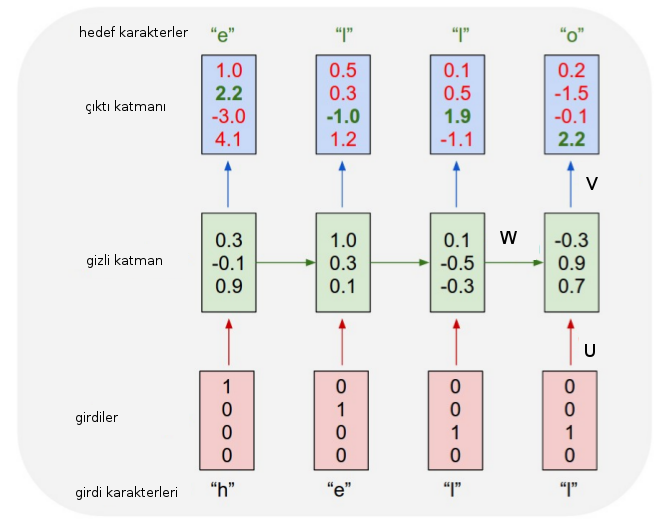
\includegraphics[width=30em]{rnn_01.png}

Daha önce işlediğimiz Öne Doğru Beslemeli (Feed-Forward) YSA'lar en temel,
klasik yapılardır. Eğer bir $N$ boyutlu girdi alıyorlarsa bu verinin tüm
boyutlarını aynı anda işlerler. RNN için [3] yapı şöyle değişiyor (tek bir
nöron için),

$x_t$: $t$ anındaki girdi. 

$s_t$: $t$ anındaki gizli konum. 

$$ s_t = f(U x_t +  W s_{t-1})$$

$o_t$: $t$ anındaki çıktı, $o_t = g(V s_t)$

İlginç olan $U,V,W$ ağırlık matrislerinin, parametrelerinin her zaman anı,
her veri noktası için aynı olması. Yani farklı zaman dilimleri için farklı
ağırlıklar atanmıyor. $t$ anındaki gizli (hidden) konum $s_t$, bu bir nevi
``hafıza''. Bu fonksiyon $x_t$ girdisinin $W$ ile çarpılması, artı bir
önceki konumun bir başka $W$ ile çarpılması sonucundan elde ediliyor. $W$
matrisi geçmişe ne kadar önem verileceğini tanımlıyorlar. Ardından tüm
hesap bir $\phi$ ile ``eziliyor'' yani belli aralıklara düşmesi zorlanıyor,
bunun için tipik olarak sigmoid, ya da $tanh$ kullanılır.

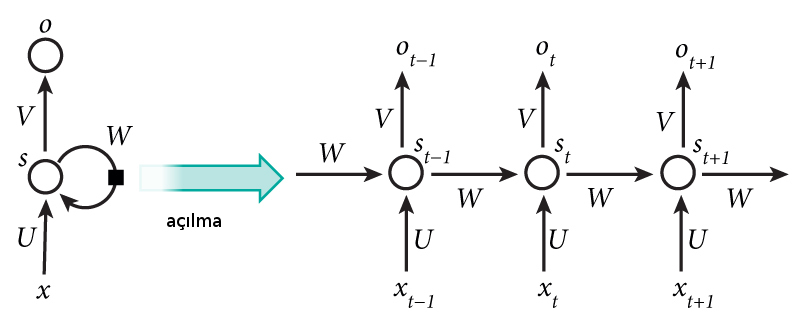
\includegraphics[width=30em]{rnn_07.jpg}

Bu kavramlar, konumlararası geçiş, $t$ anındaki girdilerin ondan önceki
girdileri nasıl bağlı olduğunun ağırlıklar üzerinden ayarlanması, yani
filtrelenmesi, aslında Markov zincirlerine benziyor (diğer bir açıdan
benzemiyor çünkü MZ matematiğinde bir zaman sadece bir öncekinden
etkilenir, RNN durumunda en baştaki adım en sondakini etkileyebilir
[4]). Bu hesaplar sonucu elde edilen tahmin ve hata geriye yayma
(backpropagation) ile ağırlık matrislerini değiştirmek için kullanılacak.

RNN ismindeki ``tekrarlanma'' $U,V,W$'nin her zaman adımı için aynı
olmasından geliyor. Ağ bir bakıma tek bir seviye için, bir kez
tanımlanıyor, ve geriye ne kadar gidileceği üzerinden o yöne doğru
kopyalanıyor, ya da ``açılıyor (unfolding)''.  Bu açılma işlemini her zaman
adımı için gösterebiliriz.  f Zaman İçinde Geriye Doğru Yayılma
(Backpropagation Through Time -BPTT-)

RNN Çesitleri, Numaraları

İlla her biriminin çıktısını kullanmak gerekmez. Her RNN biriminin $h$
formundaki gizli katman çıktısı bir sonraki birime girdi kabul edildiği
için bu çıktılar RNN'nin bütününü etkilerler, fakat etiket / düzeltme
bağlamında direk kullanılmaları şart değildir. Mesela bir RNN'e bir veri
dizisi verip, çıktılarının en sonuncusu hariç geri kalanlarını yok
sayabiliriz, o zaman bir dizi-vektör RNN'i elde ederiz. Ya da RNN'e bir
film hakkındaki tüm yorumları kelime kelime veri dizisi olarak verebiliriz,
RNN'in tek çıktısı -1/+1 şeklinde beğendi / beğenmedi skoru olabilir, bu
ünlü hissiyat analizi (sentiment analyis) örneğidir. Altta diyagramı
görüyoruz,

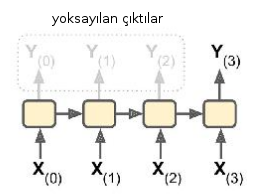
\includegraphics[width=15em]{rnn_05.png}

Eğer zaman serisi tahmin etmek istiyorsak $x_1,x_2,..$ serisini alıp bir
kaydırarak ona karşılık olan ``etiketleri'' kendimiz yaratabiliriz. Bu
durumda $y_1,y_2,..$ serisi $x_2,x_3,..$ serisi haline gelir.

Bir RNN'in tekrar eden kısım bir nöron yerine bir katman da olabilir, yani
bu katman içinde birden fazla nöron olur, ve bu katman zamanda geriye doğru
kopyalanır. 

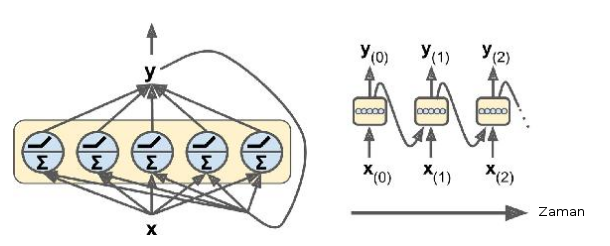
\includegraphics[width=24em]{rnn_06.png}

Eğer tüm çeşitleri göstermek gerekirse

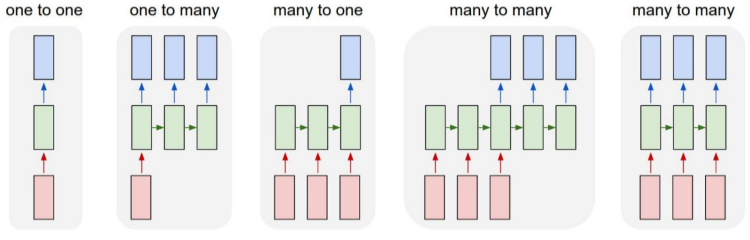
\includegraphics[width=35em]{rnn_08.png}

Bire bir (one to one) çok basit, diğerleri bire çok (one to many), çoka bir
(many to one), ve iki çeşit çoka çok (many to many). RNN yapısındaki tek
sınır herhalde tekrarlanan hücrelerden daha fazla girdi hücresi olamayacak
olması, fakat onun haricinde neredeyse her tür olasılık mümkün. Mesela
soldan 4. örnekte üç boyutlu bir girdi sadece ilk üç tekrarlanan hücreye
veriliyor, geri kalanlara bir şey verilmiyor, çıktı ise son üç hücreden
alınıyor.

Şimdi TensorFlow ile en basit RNN'yi kendimiz yaratalım. Tekrar eden bir
katman olacak, içinde 5 tane nöron,

\begin{minted}[fontsize=\footnotesize]{python}
import tensorflow as tf

def reset_graph(seed=42):
    tf.reset_default_graph()
    tf.set_random_seed(seed)
    np.random.seed(seed)

reset_graph()

n_inputs = 3
n_neurons = 5

X0 = tf.placeholder(tf.float32, [None, n_inputs])
X1 = tf.placeholder(tf.float32, [None, n_inputs])

W = tf.Variable(tf.random_normal(shape=[n_inputs, n_neurons],dtype=tf.float32))
U = tf.Variable(tf.random_normal(shape=[n_neurons,n_neurons],dtype=tf.float32))
b = tf.Variable(tf.zeros([1, n_neurons], dtype=tf.float32))

Y0 = tf.tanh(tf.matmul(X0, W) + b)
Y1 = tf.tanh(tf.matmul(Y0, U) + tf.matmul(X1, W) + b)

init = tf.global_variables_initializer()
\end{minted}

Şimdi iki veri noktası verip iki veri noktası çıktısına bakalım. Bu 2-2
verisinden pek çok olacak, ki bu veriler ufak toptan setimizi (minibatch)
oluşturacak. Alttaki ufak veride 4 tane o şekilde veri noktası var.

\begin{minted}[fontsize=\footnotesize]{python}
import numpy as np

# ufak toptan veri
X0_batch = np.array([[0, 1, 2], [3, 4, 5], [6, 7, 8], [9, 0, 1]]) # t = 0
X1_batch = np.array([[9, 8, 7], [0, 0, 0], [6, 5, 4], [3, 2, 1]]) # t = 1

with tf.Session() as sess:
    init.run()
    Y0_val, Y1_val = sess.run([Y0, Y1], feed_dict={X0: X0_batch, X1: X1_batch})

print 't=0'
print(Y0_val)
print 't=1'
print(Y1_val)
\end{minted}

\begin{verbatim}
t=0
[[-0.0664006   0.96257669  0.68105787  0.70918542 -0.89821595]
 [ 0.9977755  -0.71978885 -0.99657625  0.9673925  -0.99989718]
 [ 0.99999774 -0.99898815 -0.99999893  0.99677622 -0.99999988]
 [ 1.         -1.         -1.         -0.99818915  0.99950868]]
t=1
[[ 1.         -1.         -1.          0.40200216 -1.        ]
 [-0.12210433  0.62805319  0.96718419 -0.99371207 -0.25839335]
 [ 0.99999827 -0.9999994  -0.9999975  -0.85943311 -0.9999879 ]
 [ 0.99928284 -0.99999815 -0.99990582  0.98579615 -0.92205751]]
\end{verbatim}

Dikkat, eğitim yapmadık, ayrıca çıktı da üretmedik, sadece her basamak için
gizli katmanı hesapladık, ve RNN'e ileri yönde hesap yaptırdık, dört kez
$x_0,x_1$ verdik o da bize dört tane $y_0,y_1$ verdi. RNN'i eğitiyor
olsaydık üretilen dört $y_0,y_1$ için $V$ ile çarpım, onu ``gerçek''
veriyle / etiketlerle karşılaştırmamız gerekecekti, onun üzerinden düzeltme
yapacaktık, vs.

Üstteki kod kolaydı, fakat RNN iki yerine 100 zaman adımı geriye gitsin
isteseydik, bu çizit çok daha büyük olurdu. O tür kodları kolaylaştırmak
için TF'in özel çağrıları var, mesela \verb!static_rnn! bunlardan
biri. Üstteki ağı bu şekilde yaratabiliriz,

\begin{minted}[fontsize=\footnotesize]{python}
reset_graph()

X0 = tf.placeholder(tf.float32, [None, n_inputs])
X1 = tf.placeholder(tf.float32, [None, n_inputs])

basic_cell = tf.contrib.rnn.BasicRNNCell(num_units=n_neurons)
output_seqs, states = tf.contrib.rnn.static_rnn(basic_cell, [X0, X1],
                                                dtype=tf.float32)
Y0, Y1 = output_seqs

print 't=0'
print(Y0_val)
print 't=1'
print(Y1_val)
\end{minted}

\begin{verbatim}
t=0
[[-0.0664006   0.96257669  0.68105787  0.70918542 -0.89821595]
 [ 0.9977755  -0.71978885 -0.99657625  0.9673925  -0.99989718]
 [ 0.99999774 -0.99898815 -0.99999893  0.99677622 -0.99999988]
 [ 1.         -1.         -1.         -0.99818915  0.99950868]]
t=1
[[ 1.         -1.         -1.          0.40200216 -1.        ]
 [-0.12210433  0.62805319  0.96718419 -0.99371207 -0.25839335]
 [ 0.99999827 -0.9999994  -0.9999975  -0.85943311 -0.9999879 ]
 [ 0.99928284 -0.99999815 -0.99990582  0.98579615 -0.92205751]]
\end{verbatim}

YSA'lar kendini tekrarlayan olsun ya da olmasın aslında $f(g(h(x)))$
şeklinde basit içiçe fonksiyondurlar. Klasik YSA'da en sondaki hata
backprop ile ağırlıklardaki değişim girdiler yönünde geriye doğru yayılır,
bunu yapmak için $-\frac{\partial E}{\partial w}$ hesaplanır, böylece tüm
ağırlıklar hataya yaptıkları katkı (!) bağlamında değişikliğe uğrarlar,
``düzeltilirler'', yani düzeltme Zincir Kanunu ile dış fonksiyonlardan içe
doğru aktarılmış olur.

RNN'de içiçe olma durumu zaman faktöründen kaynaklanıyor, fonksiyonlar
önceki zaman dilimleri bağlamında içiçe geçmiş durumdadırlar, çünkü bir $t$
anındaki tahmin önceki dilimlerdeki fonksiyonların sonucudur, bir
geribesleme durumu vardır, her gizli konum $h_t$ sadece bir önceki
$h_{t-1}$ değil ondan önceki tüm gizli konumlardan da etkilenir. O zaman
eğitimin bunu gözönüne alması gerekir.

Dikkat: RNN'lerde içiçe geçen fonksiyonlar sebebiyle hatalar ya çok büyüyüp
ya da çok küçülebiliyor, normal derin YSA'lerde de problem olabilir bu,
fakat RNN'lerde bu durum daha belirgin çünkü N adım geriye gitmek demek N
kadar içiçe geçen fonksiyon demek, ve sıralı veriyi tahmin için N'in büyük
olması gerekebilir.

Örnek

Alttaki kodda bir metin okunarak o metindeki harf sırası tahmin edilmeye
uğraşılıyor. Metin tekrar sıfırdan üretilmeye çabalanıyor. Otomatik türev
(automatic differentiation -AD-) alma ile içiçe geçmiş fonksiyonların
zincirleme türevinin alınması sağlanıyor, \verb!rnn_predict! hesabı 40
geriye gider, AD tüm bu zinciri takip eder.

\inputminted[fontsize=\footnotesize]{python}{rnn.py}

\begin{minted}[fontsize=\footnotesize]{python}
import autograd.numpy as np
import autograd.numpy.random as npr
from autograd import grad
from autograd.optimizers import adam
import rnn

def build_dataset(filename, sequence_length, alphabet_size, max_lines=-1):
    with open(filename) as f:
        content = f.readlines()
    content = content[:max_lines]
    content = [line for line in content if len(line) > 2]   
    seqs = np.zeros((sequence_length, len(content), alphabet_size))
    for ix, line in enumerate(content):
        padded_line = (line + " " * sequence_length)[:sequence_length]
        seqs[:, ix, :] = string_to_one_hot(padded_line, alphabet_size)
    return seqs

num_chars = 128
text_filename = 'rnn.py'
train_inputs = build_dataset(text_filename, sequence_length=30,
                                 alphabet_size=num_chars, max_lines=60)

init_params = rnn.create_rnn_params(input_size=128, output_size=128,
                                    state_size=40, param_scale=0.01)
                                    
def print_training_prediction(weights):
    print("Training text                         Predicted text")
    logprobs = np.asarray(rnn_predict(weights, train_inputs))
    for t in range(logprobs.shape[1]):
        training_text  = one_hot_to_string(train_inputs[:,t,:])
        predicted_text = rnn.one_hot_to_string(logprobs[:,t,:])
        print(training_text.replace('\n', ' ') + "|" +
              predicted_text.replace('\n', ' '))

def callback(weights, iter, gradient):
    if iter % 10 == 0:
        print("Iteration", iter, "Train loss:", training_loss(weights, 0))
        #print_training_prediction(weights)

# Build gradient of loss function using autograd.
training_loss_grad = grad(training_loss)

print("Training RNN...")
trained_params = adam(training_loss_grad, init_params, step_size=0.1,
                      num_iters=280, callback=callback)
\end{minted}

\begin{verbatim}
Training RNN...
('Iteration', 0, 'Train loss:', 4.854500980126768)
('Iteration', 10, 'Train loss:', 3.069896973468059)
('Iteration', 20, 'Train loss:', 2.9564946588218)
('Iteration', 30, 'Train loss:', 2.590610887049078)
('Iteration', 40, 'Train loss:', 2.3255385285729027)
('Iteration', 50, 'Train loss:', 2.1211122619024696)
('Iteration', 60, 'Train loss:', 1.9691676257416404)
('Iteration', 70, 'Train loss:', 1.8868756780002685)
('Iteration', 80, 'Train loss:', 1.7455098359656291)
('Iteration', 90, 'Train loss:', 1.7750342336507772)
('Iteration', 100, 'Train loss:', 1.6059292555729703)
('Iteration', 110, 'Train loss:', 1.5077116694554635)
('Iteration', 120, 'Train loss:', 1.437485110908115)
('Iteration', 130, 'Train loss:', 1.4504849515039933)
('Iteration', 140, 'Train loss:', 1.3480379515887519)
('Iteration', 150, 'Train loss:', 1.4083643059429929)
('Iteration', 160, 'Train loss:', 1.2655987546227996)
('Iteration', 170, 'Train loss:', 1.2051278365327054)
('Iteration', 180, 'Train loss:', 1.1561998913079512)
('Iteration', 190, 'Train loss:', 1.1814640952544757)
('Iteration', 200, 'Train loss:', 1.3673188298901471)
('Iteration', 210, 'Train loss:', 1.1591863193874781)
('Iteration', 220, 'Train loss:', 1.056688128805028)
('Iteration', 230, 'Train loss:', 1.0465201536978259)
('Iteration', 240, 'Train loss:', 1.0373081053464259)
('Iteration', 250, 'Train loss:', 1.3591698106017474)
('Iteration', 260, 'Train loss:', 1.1556108786809474)
('Iteration', 270, 'Train loss:', 1.0323757883394502)
\end{verbatim}

Üretmek / eğitim için \verb!rnn.py! kodunun kendisi kullanıldı.

\begin{minted}[fontsize=\footnotesize]{python}
num_letters = 30
for t in range(20):
    text = ""
    for i in range(num_letters):
        seqs = rnn.string_to_one_hot(text, num_chars)[:, np.newaxis, :]
        logprobs = rnn.rnn_predict(trained_params, seqs)[-1].ravel()
        text += chr(npr.choice(len(logprobs), p=np.exp(logprobs)))
    print(text)
\end{minted}

\begin{verbatim}
    rs.lepugnunpdit - cenedili
def p.rnns, logs'ininpum, hid_
    ngan rrad_ti, feturn ns.sc
def catorrtar t  aut_re_strad.
            hiddens_numumut in
def hiddes = rhiddensdord.rato
    return ncan((ponddens_tram
ders minpperen(scnt_strt onut_
    returnts, utete, jIoutdati
    return oute_sthorn(pund_om
dershgline nigms, conteme_sco_
    return 0.5*(natorad.mincde
    contse, hiddens_mihrra opu
    [cran_put inhgto_tut= retu
  # Ite, wItre =        retat 
    ashis_lik[enutnoncam(nthen
      oonname, jItogput_pre_sp
    cet(fiddens = lot led_ome_
def rinnam_idt(parddens_nnd(on
    rs.leteqslind_tat  = [hipp
\end{verbatim}

Fena değil; \verb!def! ile başlanan satır ardından sonraki satır tab ile
boşluk bıraktı, bunlar kolay şeyler değil.  Altta karşılaştırma amaçlı
olarak sadece frekans sayarak üretim yapan bir kod görüyoruz. O da fena
değil, bu konu hakkında daha fazla detay için [2].

\begin{minted}[fontsize=\footnotesize]{python}
f = "../../stat/stat_naive/data/a1.txt"
print open(f).read()[:300]
\end{minted}

\begin{verbatim}
A well-known scientist (some say it was Bertrand Russell) once gave a
public lecture on astronomy. He described how the earth orbits around
the sun and how the sun, in turn, orbits around the center of a vast
collection of stars called our galaxy. At the end of the lecture, a
little old lady at the 
\end{verbatim}

\begin{minted}[fontsize=\footnotesize]{python}
import lm
lmm = lm.train_char_lm(f, order=4)
res = lm.generate_text(lmm, 4)
print res[:400]
\end{minted}

\begin{verbatim}
A well-know
better? What the moon were caused by Ptolemy in more the picture only late the Greeks even had
been elongstanding that the sky what eclipses rather ridiculous, but why do we know about to someone looking the sun and the earth Star
lies one looking the North orbiting questimate thought spheres the superior smile before think we go back of the really a flat plater see then? What disk, th
\end{verbatim}


\begin{minted}[fontsize=\footnotesize]{python}
print lmm.keys()[:10]
print lmm.get('pla')
\end{minted}

\begin{verbatim}
['t w', 'Fir', 'all', 't t', 'sci', 'rom', 'ron', 'roo', 'thi', 'oss']
[('t', 0.5), ('n', 0.5)]
\end{verbatim}

Zaman Serisi Tahmini

Tensorflow ile zaman serisi tahmini yapalım. Eğitim verisinin formülünü
bildiğimiz bir sinüs eğrisinden alacağız, sanki eğriyi bilmiyormuş gibi
yapalım, bu eğriyi sadece üretilen veriye bakarak ``öğreneceğiz''. Eğrinin
rasgele kısımlarından toptan veri parçaları üretmek için bir çağrı yazalım,

\begin{minted}[fontsize=\footnotesize]{python}
np.random.seed(1)

t_min, t_max = 0, 30
resolution = 0.1

def f(t):
    return t * np.sin(t) / 3 + 2 * np.sin(t*5)

def next_batch(batch_size, n_steps):
    t0 = np.random.rand(batch_size, 1) * (t_max - t_min - n_steps * resolution)
    Ts = t0 + np.arange(0., n_steps + 1) * resolution
    ys = f(Ts)
    return ys[:, :-1].reshape(-1, n_steps, 1), ys[:, 1:].reshape(-1, n_steps, 1)
\end{minted}

Eğitim verisi zaman serisinin ufak bir parçası, ve hedef verisi onun bir
ileri kaydırılmış hali. 

Zaman serisinin rasgele şekilde nasıl örneklendiğini göstermek için üstteki
çağrı içindeki örnekleme kodunun benzerini altta tekrarlayalım ve
grafikleyelim. Kırmızı noktalar örneklenen veri noktaları,

\begin{minted}[fontsize=\footnotesize]{python}
batch_size = 5
n_steps = 3
t0 = np.random.rand(batch_size, 1) * (t_max - t_min - n_steps * resolution)
Ts = t0 + np.arange(0., n_steps+1) * resolution
ys = f(Ts)
print ys
\end{minted}

\begin{verbatim}
[[-2.3141651  -1.12233854  0.27200624  1.6253068 ]
 [ 4.31878159  4.63599743  4.61528818  4.112844  ]
 [ 0.03397153  0.99207952  1.71474727  2.02731967]
 [ 2.87376693  3.00044595  2.62695206  1.77847377]
 [-0.96970753 -2.03368272 -2.93926439 -3.47887785]]
\end{verbatim}

Grafiklersek,

\begin{minted}[fontsize=\footnotesize]{python}
t = np.linspace(t_min, t_max, int((t_max - t_min) / resolution))
y = f(t)
plt.plot(t,y)
plt.plot(Ts,ys,'r.')
plt.savefig('rnn_03.png')
\end{minted}

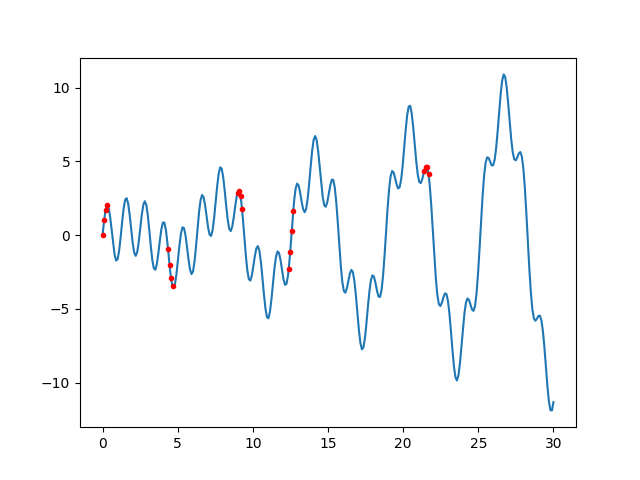
\includegraphics[width=20em]{rnn_03.png}

Öğrenme amacıyla daha büyük adım, iç nöron sayısı tanımlayalım,

\begin{minted}[fontsize=\footnotesize]{python}
import tensorflow as tf

def reset_graph(seed=42):
    tf.reset_default_graph()
    tf.set_random_seed(seed)
    np.random.seed(seed)

reset_graph()

n_steps = 30
n_inputs = 1
n_neurons = 200
n_outputs = 1

X = tf.placeholder(tf.float32, [None, n_steps, n_inputs])
y = tf.placeholder(tf.float32, [None, n_steps, n_outputs])

cell = tf.contrib.rnn.OutputProjectionWrapper(
    tf.contrib.rnn.BasicRNNCell(num_units=n_neurons, activation=tf.nn.relu),
    output_size=n_outputs)

outputs, states = tf.nn.dynamic_rnn(cell, X, dtype=tf.float32)

learning_rate = 0.01

loss = tf.reduce_mean(tf.square(outputs - y)) # MSE
optimizer = tf.train.AdamOptimizer(learning_rate=learning_rate)
training_op = optimizer.minimize(loss)

init = tf.global_variables_initializer()

n_iterations = 300
batch_size = 50

sess = tf.Session()

sess.run(tf.global_variables_initializer())

for iteration in range(n_iterations):
    X_batch, y_batch = next_batch(batch_size, n_steps)
    sess.run(training_op, feed_dict={X: X_batch, y: y_batch})
    if iteration % 100 == 0:
        mse = loss.eval(feed_dict={X: X_batch, y: y_batch}, session=sess)
        print(iteration, "\tMSE:", mse)

\end{minted}

\begin{verbatim}
(0, '\tMSE:', 280.63486)
(100, '\tMSE:', 0.089582793)
(200, '\tMSE:', 0.044634577)
\end{verbatim}

Öğrenme tamamlandı ve MSE hata raporu fena değil. Şimdi bu RNN'i hiç
görmediğimiz geleceği tahmin için kullanalım, \verb!n_more! adım ilerisini
tahmin edeceğiz, yanlız \verb!n_steps! zaman serisi kaydırılmış
\verb!n_steps! ilerisini tahmin için kullanılıyordu. Biz tahminleri
üretirken tahmin bloğunun sadece en sondaki öğesini alacağız. Sonra bu
ögeyi kaynak veriye dahil edip bir gelecek bloğu daha üreteceğiz (onun da
son öğesini alacağız, vs), ve böyle gide gide \verb!n_more! kadar geleceği
bitiştirmiş olacağız. 

\begin{minted}[fontsize=\footnotesize]{python}
n_more = 40

t = np.linspace(t_min, t_max, int((t_max - t_min) / resolution))
y = f(t)

newx = list(t[-n_steps:])
newy = list(y[-n_steps:])
for i in range(n_more): # bu kadar daha uret
   tst_input = np.array(newy[-n_steps:]).reshape(1,n_steps,1) 
   res = sess.run(outputs, feed_dict={X: tst_input})
   newy.append(res[0][0][0])
   newx.append(t_max + (i*resolution))

plt.plot(t,y)
plt.plot(newx[n_steps-1:],newy[n_steps-1:],'g')

plt.savefig('rnn_04.png')
\end{minted}

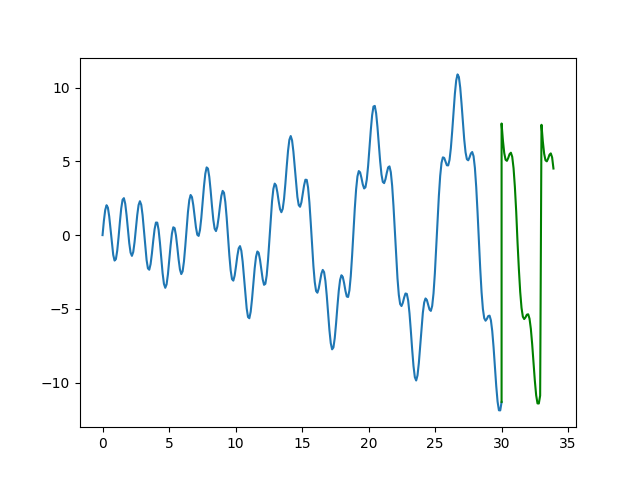
\includegraphics[width=20em]{rnn_04.png}

Yeşil renkli tahmin bölümü. 

Problemler

RNN problemlerinden biri şerisel olarak modellenen verinin ağ yapısında
geriye doğru giderken eğitim sırasında yokolan gradyan (vanishing gradient)
problemine sebep olabilmesi. Çünkü YSA yatay olarak derin, ve gradyan
geriye doğru yayılma yaparken sayısal olarak problemlere yol
açabiliyor. Çözümler adım sayısını azaltmak olabilir, ya da bu problemlerin
bazılarını düzelten LSTM kullanmak olabilir.

Kaynaklar

[1] {\em A Beginner's Guide to Recurrent Networks and LSTMs}, 
    \url{https://deeplearning4j.org/lstm#a-beginners-guide-to-recurrent-networks-and-lstms}

[2] Bayramlı, 
    {\em Derin Öğrenim ile Text Üretmek, RNN, LSTM}, 
    \url{https://burakbayramli.github.io/dersblog/sk/2017/01/derin-ogrenim-ile-text-uretmek-rnn-lstm.html}

[3] Britz, {\em Recurrent Neural Networks Tutorial, Part 1}, \url{http://www.wildml.com/2015/09/recurrent-neural-networks-tutorial-part-1-introduction-to-rnns/}

[4] Lipton, {\em A Critical Review of Recurrent Neural Networks for Sequence Learning},\url{https://arxiv.org/abs/1506.00019}


\end{document}
